\section{Faisal Najib Abdullah / 1174042}
\subsection{Teori}

\begin{enumerate}

\item Jelaskan Kenapa file teks harus dilakukan tokenizer. Dilengkap dengan ilustrasi atau gambar.\par
Tokenizer adalah proses untuk membagi kalimat menjadi beberapa teks, hal ini sangat di perlukan dalam AI karena nanti setiap teks akan di hitung bobotnya dang akan memunculkan nilai vektor sehingga teks tersebut bisa di gunakan sebagai data untuk memprediksi teks yang muncul dalam satu kalimat sedangakan proses tkenizer merupakan caramembagi bagi teks dari suatu kalimat biasanya pembagi kalimat tersebut merupakan spasi dalan suatu kalimat.
\begin{figure}[ht]
\centering
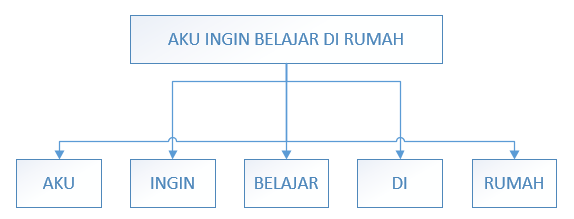
\includegraphics[scale=0.4]{figures/1174042/chapter7/1,1.PNG}
\caption{Ilustrasi Tokenisasi}
\label{Contoh}
\end{figure}


\item jelaskan konsep dasar K Fold Cross VAlidation dan dataset komentar youtube pada code berikut dilengkapi dengan ilustrasi gambar  
\begin{verbatim}
kfold = StartifiedKFlod(n_splits=5)
splits = kfold.split(d, d['CLASS'])
\end{verbatim}
pada codingan tersebut terdapat kfold sebagai variabel yang didalammnya terdiri dari split 5 yang berarti pengulangan terhadap pengolahan masing masing lima kali pada kasus ini terdapat data sebanyak 5 berarti ke lima data tersebut di ulang sebanyak lima kali dengan atribut class sebagai acuan pengolahan datanya kemudian akan di hasilkan akurasi dari pengulangan data tersebut sebesar sekian persen tergantung datanya.
\begin{figure}[ht]
\centering
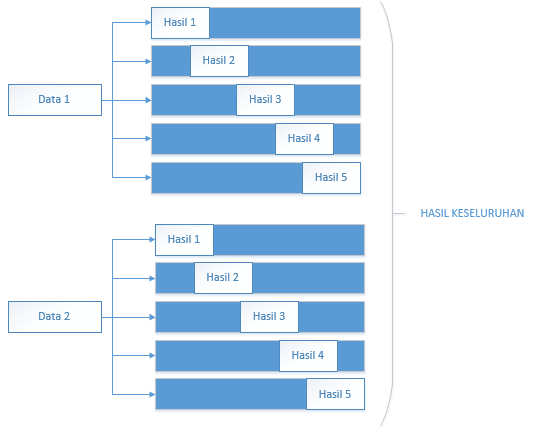
\includegraphics[scale=0.4]{figures/1174042/chapter7/1,2.PNG}
\caption{Ilustrasi K Fold Cross Validation}
\label{Contoh}
\end{figure}


\item Jelaskan apa maksudnya kode program for train, test in split dilengkapi di lengkapi dengan ilustrasi atau gambar.\par
for train di gunakan melakukan training atau pelatihan terhadap data yang telah di deklarasikan sebelumnya. sedangkan test in split di gunakan untuk diguanakan untuk membatasi jumlah data yang akan di inputkan atau data yang akan di gunakan.
\begin{figure}[ht]
\centering
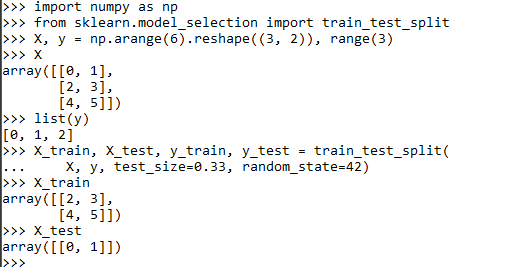
\includegraphics[scale=0.4]{figures/1174042/chapter7/1,3.PNG}
\caption{Ilustrasi For Train dan Test in split}
\label{Contoh}
\end{figure}


\item Jelaskan apa maksud kode program traint\_content =d['CONTENT'].iloc[traint\_idx] dan test\_content =d['CONTENT'].iloc[traint\_idx]. dilengkapi dengan ilustrasi atau gambar.\par
maksud dari kode program tersebut adalah membaca isian kolom pada field yang bernama CONTENT sebagai data training dan data testing untuk program tersebut.
\begin{figure}[ht]
\centering
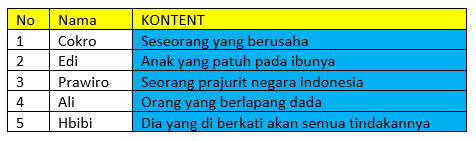
\includegraphics[scale=0.4]{figures/1174042/chapter7/1,4.PNG}
\caption{Ilustrasi Penggunaan kolom CONTENT}
\label{Contoh}
\end{figure}


\item Jelaskan maksud dari fungsi tokenizer = Tokennizer(num\_words=2000)dan tokenizer.fit\_on\_texts(train\_konten) di lengkapi dengan ilustrasi gambar.\par
fungsi tokenizer = Tokennizer(num\_words=2000) digunakan untuk membaca kalimat yang telah di buat menjadi token sebanyak 2000 kata dan fingsi fit\_on\_texts(train\_konten) digunakan untuk membuat membaca data token teks yang telah di masukan kedalam fungsi yaitu fungsi train\_konten.
\begin{figure}[ht]
\centering
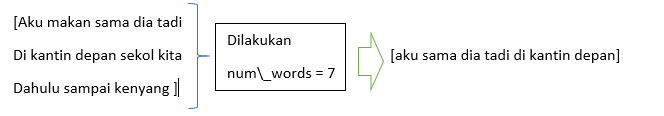
\includegraphics[scale=0.4]{figures/1174042/chapter7/1,5.PNG}
\caption{Ilustrasi fit tokenizer dan num\_word=2000}
\label{Contoh}
\end{figure}


\item Jelaskan apa maksud dari fungsi d train inputs = tokenizer.texts to matrix(train content, mode=tfidf) dan d test inputs = tokenizer.texts to matrix(test content, mode=tfidf), dilengkapi dengan ilustrasi kode dan atau gambar.\par 
yaitu di gunakan untuk mengubah urutan teks yang tadi telah di lakukan tokenizer menjadi matriks yang berut=rutan seperti tf idf 
\begin{figure}[ht]
\centering
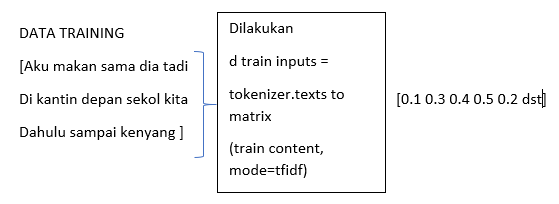
\includegraphics[scale=0.4]{figures/1174042/chapter7/1,6.PNG}
\caption{Ilustrasi d train inputs = tokenizer.texts to matrix(train content, mode=tfidf)}
\label{Contoh}
\end{figure}


\item Jelaskan apa maksud dari fungsi \emph{d\_train\_inputs = d\_train\_inputs/np.amax(np.absolute(d\_train\_inputs))} dan \emph{d\_test\_inputs = d\_test\_inputs/np.amax(np.absolute(d\_test\_inputs))}, dilengkapi dengan ilustrasi atau gambar \par

fungsi tersebut digunakan untuk membagi matriks tfidf dengan dengan penentuan maksimum aray sepanjang sumbu sehingga akan menimbulkan garis ke bawah dan keatas yang membentuk gambar v kemudian hasil tersebut akan di masukan ke dalam variabel d train input dan d test input dengan methode absolute. yang berarti tanpa bilangan negatif.
\begin{figure}[ht]
\centering
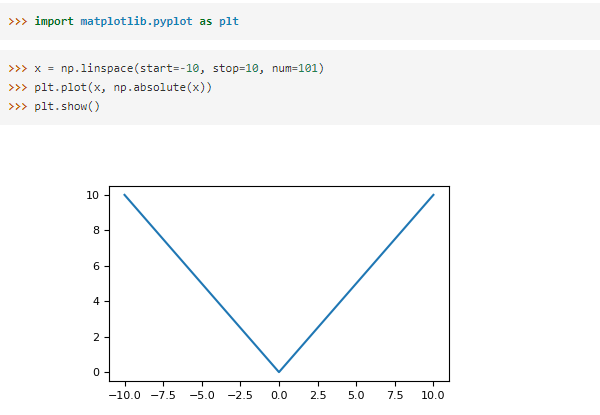
\includegraphics[scale=0.4]{figures/1174042/chapter7/1,7.PNG}
\caption{Ilustrasi d\_train\_inputs = d\_train\_inputs/np.amax(np.absolute(d\_train\_inputs))}
\label{Contoh}
\end{figure}


\item Jelaskan apa maksud fungsi dari d train outputs = np utils.to categorical(d['CLASS'].iloc[train dan d test outputs = np utils.to categorical(d['CLASS'].iloc[test idx]) dalam kode program, dilengkapi dengan ilustrasi atau gambar.\par

maksud dari fungsi tersebut yaitu untuk merubah nilai vektor yang ada pada atribut class menjadi bentuk matrix dengan pengurutan berdasarkan data index training dan testing.
\begin{figure}[ht]
\centering
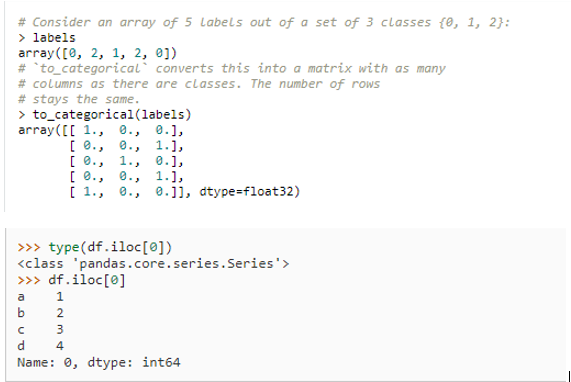
\includegraphics[scale=0.4]{figures/1174042/chapter7/1,8.PNG}
\caption{Ilustrasi train outputs = np utils.to categorical(d['CLASS'].iloc[train}
\label{Contoh}
\end{figure}


\item model = sequential berarti variabel model berisi method sequential yang berguna untuk searching data dengan menerima parameter atau argumen kunci dengan langkah tertentu untuk mencari data yang telah di olah. kemudian modeldi tambahkan metod add dengan Dense yang berarti data data yang di inputkan akan terhubung, dengan data 612 dan 2000 data  kata atau word kemudian model tersebut di masukan fungsi aktivation dengan rumusa atau methode relu setelah itu data tersebut di dropout 0.5 atau di pangkas sebanyak 50 persen di karenakan pada pohon bobot terlalu akurat terhadap data. sehingga data dilakukan pemangkasan 50 persen. kemudian data tersebut di hubungkan. setelah data tersebut di hubungkan maka di lakukan perhitungan dengan menggunakan fungsi softmax. 
\begin{figure}[ht]
\centering
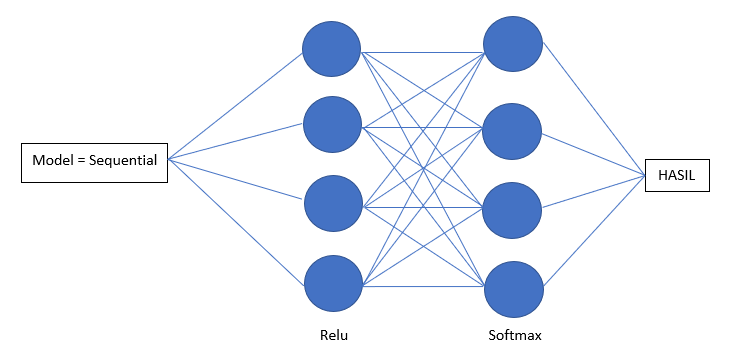
\includegraphics[scale=0.4]{figures/1174042/chapter7/1,9.PNG}
\caption{Ilustrasi Neural Network}
\label{Contoh}
\end{figure}


\item model tersebut kemudian di compile atau di kembalikan kembali fungsi nilainya yangmana akan mengembalikan fungsi nilai loss nya berapa yang diambil dari fungsi adamax yang berberguna untuk  mengetahui nilai lossnya kemudian metrics = acuracy merupakan akurasi dari nilai matrixnya.

\item Jelaskan apa itu Deep Learning \par
merupakan salah satu algoritma jaringan saraf tiruan yang menggunakan meta data sebagai inputan dan mengolahnya menggunakan layer layer yang tersembunyi. deep lerning memiliki suatu keunikan yaitu fitur yang dapat mengekstraksi secara otomatis.

\item Jelaskan Apa itu Deep Neural Network dan apa perbedaanya dengan Deep Learning.\par
merupakan algoritma jaringan syaraf juga yang mena akan melakukan pembobotan terhadap data yang sudah ada sebagai acuan untuk data inputan selanjutnya. kemudian terdiri atas beberapa layer atau hiden layer. perbedaan antara deep learning dan DNN atau Deep Neural Network yaitu deep lerning merupakan pemakai algoritma dari DNN dan DNN merupakan algoritma yang ada pada deep learning.

\item Jelaskan dengan ilustrasi gambar buatan sendiri(langkah per langkah) bagaimana perhitungan algoritma konvolusi dengan ukuran stride (NPM mod3+1) x (NPM mod3+1) yang terdapat max pooling.(nilai 30)\par
 sebelum membuat ilustrasi perlu di ketahui apa itu stride, stride adalah acuan atau parameter yang menentukan pergeseran pada filter fixcel. sebagai contoh nilai stride 1 yang berarti filter akan bergeser sebanyak satu fixcel secara vertikal dan horizontal. selanjutnya apa itu max pooling contoh pada suatu gambar di tentukan Max Pooling dari 3 x 3 dengan stride 1 yang berarti setiap pergeseran 1 pixcel akan diambil nilai terbesar dari pixcel 3 x 3 tersebut.\par

selanjutnya jawaban dari soal ini yaitu menggunakan stride 1 dengan ketentuan max pooling. 
\begin{figure}[ht]
\centering
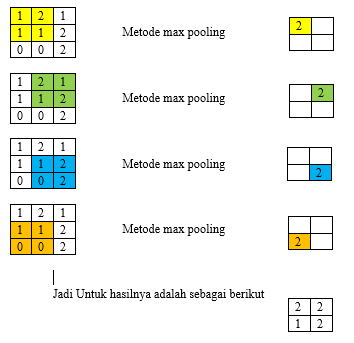
\includegraphics[scale=0.4]{figures/1174042/chapter7/1,10.PNG}
\caption{Hasil perhitungan stride 1 max pooling}
\label{Contoh}
\end{figure}

\end{enumerate}

\subsection{Pemrograman}
Penjelasan setiap baris code dari nomer 1 sampai 20 bisa di lihat pada bagian cooment coding yang berwarna hijau.
\begin{enumerate}
\item Jelaskan kode program pada blok  In[1].
\lstinputlisting{src/1174042/chapter7/2,1.py}
Untuk hasilnya dapat di lihat pada gambar berikut.
\begin{figure}[ht]
\centering
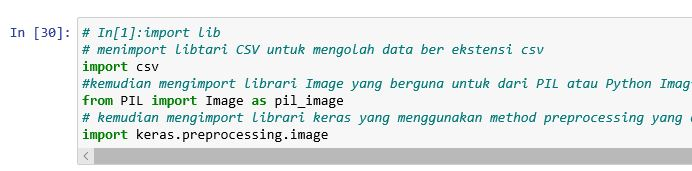
\includegraphics[scale=0.4]{figures/1174042/chapter7/2,1.JPG}
\caption{hasil kode program}
\label{Contoh}
\end{figure}


\item Jelaskan kode program pada blok  In[2].
\lstinputlisting{src/1174042/chapter7/2,2.py}
Untuk hasilnya dapat di lihat pada gambar berikut.
\begin{figure}[ht]
\centering
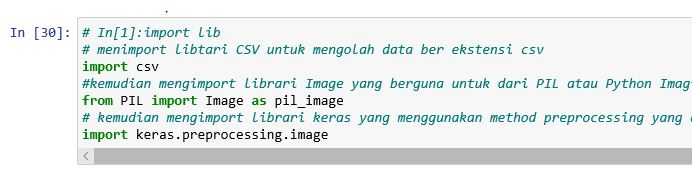
\includegraphics[scale=0.4]{figures/1174042/chapter7/2,2.JPG}
\caption{hasil kode program}
\label{Contoh}
\end{figure}


\item Jelaskan kode program pada blok  In[3].
\lstinputlisting{src/1174042/chapter7/2,3.py}
Untuk hasilnya dapat di lihat pada gambar berikut.
\begin{figure}[ht]
\centering
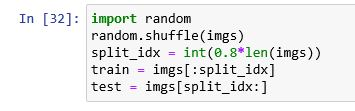
\includegraphics[scale=0.4]{figures/1174042/chapter7/2,3.JPG}
\caption{hasil kode program}
\label{Contoh}
\end{figure}

\item Jelaskan kode program pada blok  In[4].
\lstinputlisting{src/1174042/chapter7/2,4.py}
Untuk hasilnya dapat di lihat pada gambar berikut.
\begin{figure}[ht]
\centering
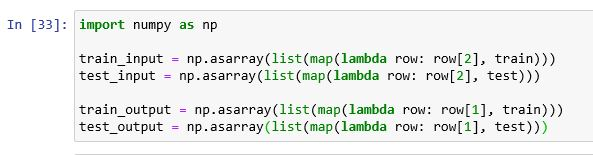
\includegraphics[scale=0.4]{figures/1174042/chapter7/2,4.JPG}
\caption{hasil kode program}
\label{Contoh}
\end{figure}

\item Jelaskan kode program pada blok  In[5].
\lstinputlisting{src/1174042/chapter7/2,5.py}
Untuk hasilnya dapat di lihat pada gambar berikut.
\begin{figure}[ht]
\centering
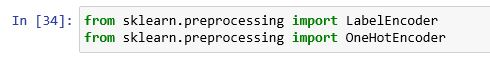
\includegraphics[scale=0.4]{figures/1174042/chapter7/2,5.JPG}
\caption{hasil kode program}
\label{Contoh}
\end{figure}

\item Jelaskan kode program pada blok  In[6].
\lstinputlisting{src/1174042/chapter7/2,6.py}
Untuk hasilnya dapat di lihat pada gambar berikut.
\begin{figure}[ht]
\centering
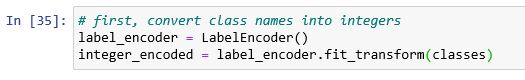
\includegraphics[scale=0.4]{figures/1174042/chapter7/2,6.JPG}
\caption{hasil kode program}
\label{Contoh}
\end{figure}

\item Jelaskan kode program pada blok  In[7].
\lstinputlisting{src/1174042/chapter7/2,7.py}
Untuk hasilnya dapat di lihat pada gambar berikut.
\begin{figure}[ht]
\centering
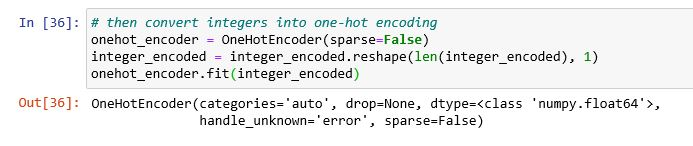
\includegraphics[scale=0.4]{figures/1174042/chapter7/2,7.JPG}
\caption{hasil kode program}
\label{Contoh}
\end{figure}

\item Jelaskan kode program pada blok  In[8].
\lstinputlisting{src/1174042/chapter7/2,8.py}
Untuk hasilnya dapat di lihat pada gambar berikut.
\begin{figure}[ht]
\centering
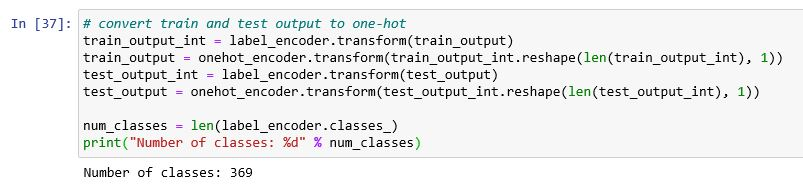
\includegraphics[scale=0.4]{figures/1174042/chapter7/2,8.JPG}
\caption{hasil kode program}
\label{Contoh}
\end{figure}

\item Jelaskan kode program pada blok  In[9].
\lstinputlisting{src/1174042/chapter7/2,9.py}
Untuk hasilnya dapat di lihat pada gambar berikut.
\begin{figure}[ht]
\centering
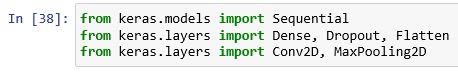
\includegraphics[scale=0.4]{figures/1174042/chapter7/2,9.JPG}
\caption{hasil kode program}
\label{Contoh}
\end{figure}

\item Jelaskan kode program pada blok  In[10].
\lstinputlisting{src/1174042/chapter7/2,10.py}
Untuk hasilnya dapat di lihat pada gambar berikut.
\begin{figure}[ht]
\centering
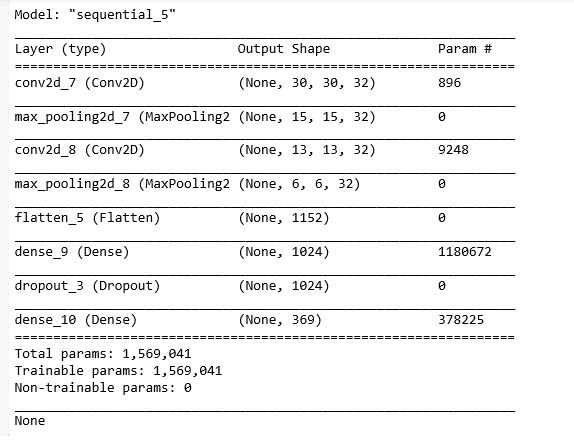
\includegraphics[scale=0.4]{figures/1174042/chapter7/2,10.JPG}
\caption{hasil kode program}
\label{Contoh}
\end{figure}

\item Jelaskan kode program pada blok  In[11].
\lstinputlisting{src/1174042/chapter7/2,11.py}
Untuk hasilnya dapat di lihat pada gambar berikut.
\begin{figure}[ht]
\centering
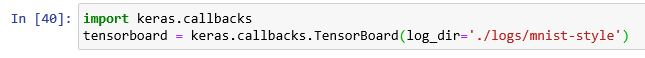
\includegraphics[scale=0.4]{figures/1174042/chapter7/2,11.JPG}
\caption{hasil kode program}
\label{Contoh}
\end{figure}

\item Jelaskan kode program pada blok  In[12].
\lstinputlisting{src/1174042/chapter7/2,12.py}
Untuk hasilnya dapat di lihat pada gambar berikut.
\begin{figure}[ht]
\centering
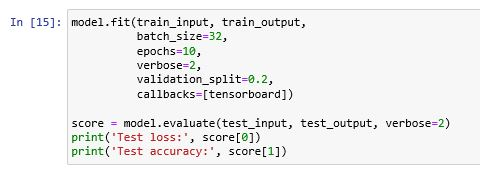
\includegraphics[scale=0.4]{figures/1174042/chapter7/2,12.JPG}
\caption{hasil kode program}
\label{Contoh}
\end{figure}

\item Jelaskan kode program pada blok  In[13].
\lstinputlisting{src/1174042/chapter7/2,13.py}
Untuk hasilnya dapat di lihat pada gambar berikut.
\begin{figure}[ht]
\centering
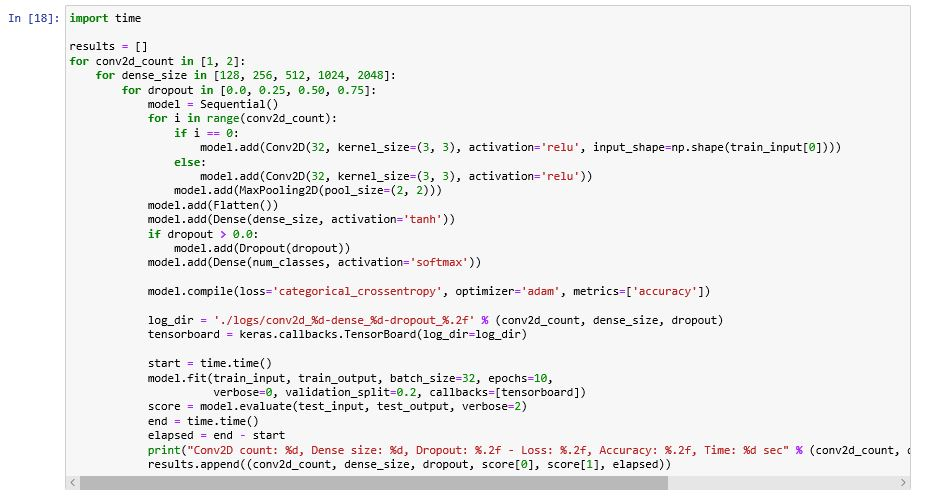
\includegraphics[scale=0.4]{figures/1174042/chapter7/2,13.JPG}
\caption{hasil kode program}
\label{Contoh}
\end{figure}

\item Jelaskan kode program pada blok  In[14].
\lstinputlisting{src/1174042/chapter7/2,14.py}
Untuk hasilnya dapat di lihat pada gambar berikut.
\begin{figure}[ht]
\centering
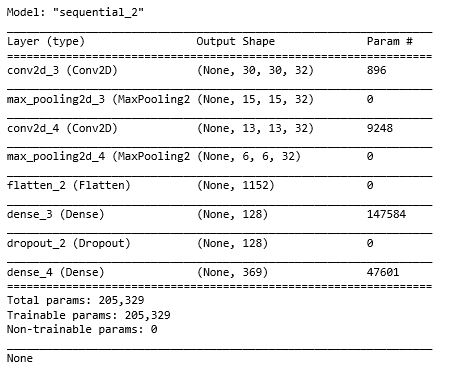
\includegraphics[scale=0.4]{figures/1174042/chapter7/2,14.JPG}
\caption{hasil kode program}
\label{Contoh}
\end{figure}

\item Jelaskan kode program pada blok  In[15].
\lstinputlisting{src/1174042/chapter7/2,15.py}
Untuk hasilnya dapat di lihat pada gambar berikut.
\begin{figure}[ht]
\centering
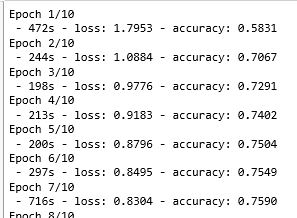
\includegraphics[scale=0.4]{figures/1174042/chapter7/2,15.JPG}
\caption{hasil kode program}
\label{Contoh}
\end{figure}

\item Jelaskan kode program pada blok  In[16].
\lstinputlisting{src/1174042/chapter7/2,16.py}
Untuk hasilnya dapat di lihat pada gambar berikut.
\begin{figure}[ht]
\centering
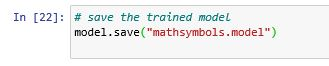
\includegraphics[scale=0.4]{figures/1174042/chapter7/2,16.JPG}
\caption{hasil kode program}
\label{Contoh}
\end{figure}

\item Jelaskan kode program pada blok  In[17].
\lstinputlisting{src/1174042/chapter7/2,17.py}
Untuk hasilnya dapat di lihat pada gambar berikut.
\begin{figure}[ht]
\centering
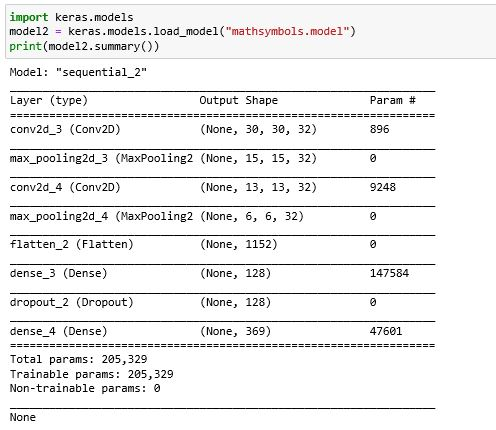
\includegraphics[scale=0.4]{figures/1174042/chapter7/2,17.JPG}
\caption{hasil kode program}
\label{Contoh}
\end{figure}

\item Jelaskan kode program pada blok  In[18].
\lstinputlisting{src/1174042/chapter7/2,18.py}
Untuk hasilnya dapat di lihat pada gambar berikut.
\begin{figure}[ht]
\centering
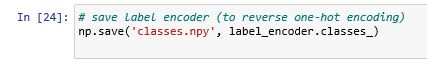
\includegraphics[scale=0.4]{figures/1174042/chapter7/2,18.JPG}
\caption{hasil kode program}
\label{Contoh}
\end{figure}

\item Jelaskan kode program pada blok  In[19].
\lstinputlisting{src/1174042/chapter7/2,19.py}
Untuk hasilnya dapat di lihat pada gambar berikut.
\begin{figure}[ht]
\centering
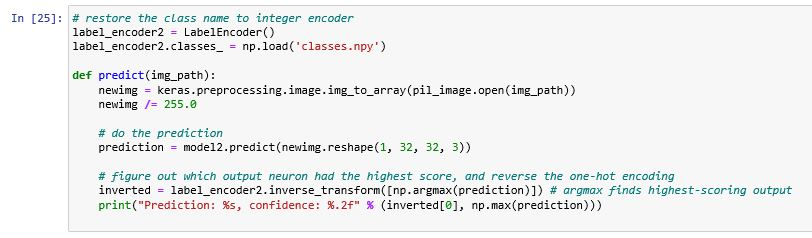
\includegraphics[scale=0.4]{figures/1174042/chapter7/2,19.JPG}
\caption{hasil kode program}
\label{Contoh}
\end{figure}

\item Jelaskan kode program pada blok  In[20].
\lstinputlisting{src/1174042/chapter7/2,20.py}
Untuk hasilnya dapat di lihat pada gambar berikut.
\begin{figure}[ht]
\centering
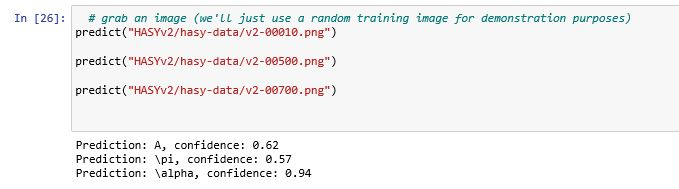
\includegraphics[scale=0.4]{figures/1174042/chapter7/2,20.JPG}
\caption{hasil kode program}
\label{Contoh}
\end{figure}

\end{enumerate}